\chapter{Problem Description}

In the present chapter the problem is presented, along with an introduction to the previous work. It is structured as follows: Section \ref{ch_2:sect:aerostack} introduces the Aerostack framework, Section \ref{ch_2:sect:requirements} presents the context of the problem and the requirements a replacement should have. Section \ref{ch_2:sect:improvements} describes deeply the improvements presented and the decisions taken to end in Section \ref{ch_2:sect:previous_work} with the description of the previous system.

  \section{The Aerostack Framework} \label{ch_2:sect:aerostack}

    Aerostack is an agnostic framework to build and design control architectures for aerial robotic systems. It provides some low level components as well as coordination processes and some planners. Figure \ref{ch_2:fig:aerostack_arqu} shows the general architecture of the framework.

    \begin{figure}[ht]
      \centering
      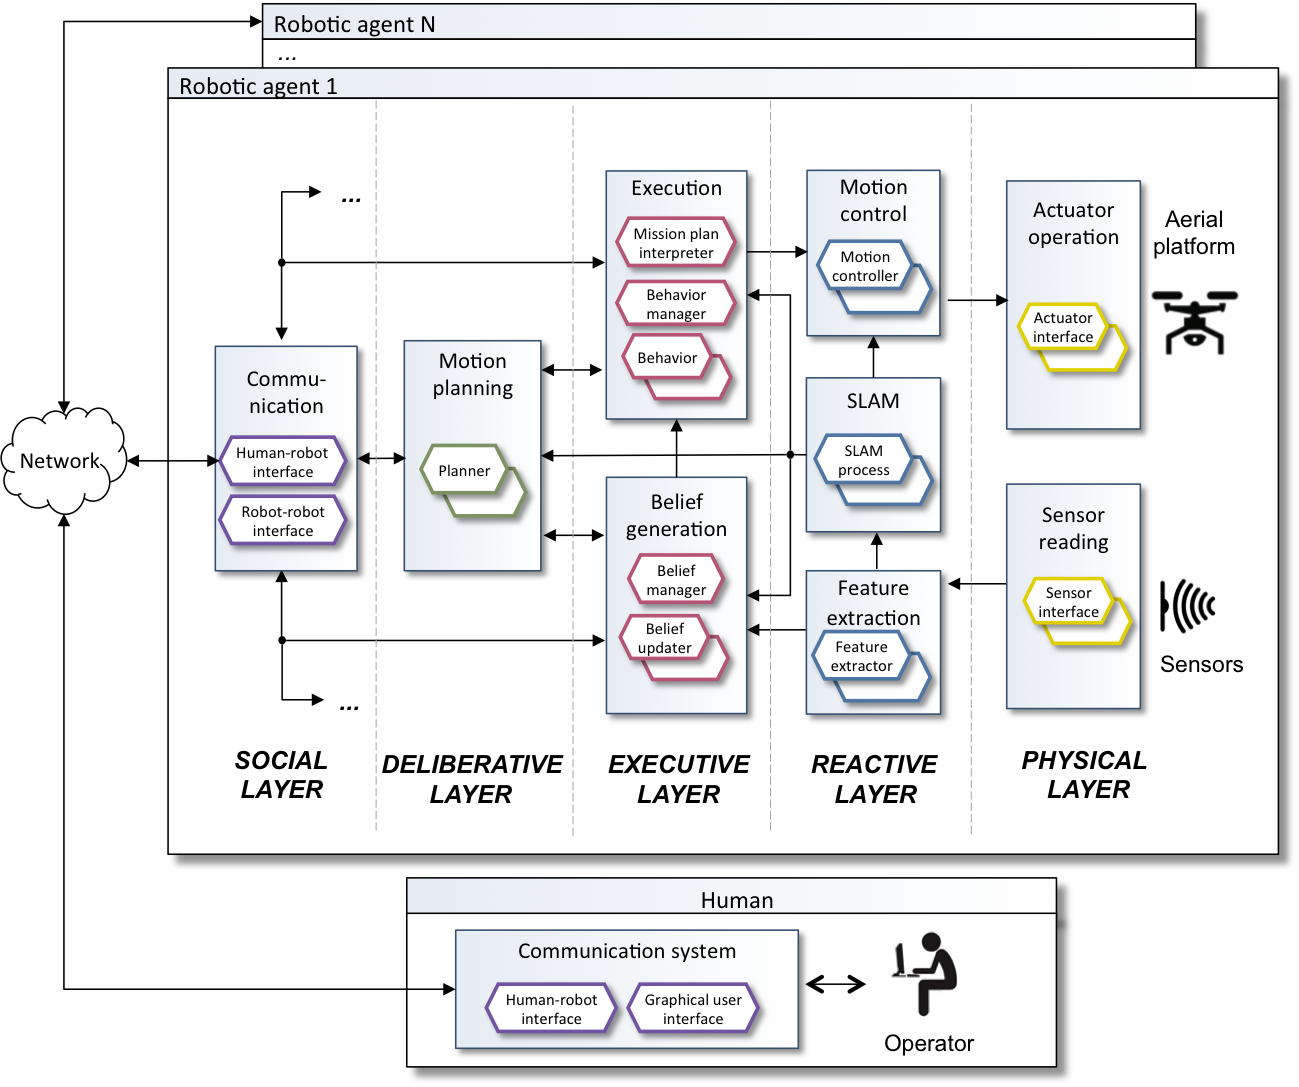
\includegraphics[width=0.8\textwidth]{AerostackArquitecture.png}
      \caption{The Aerostack architecture}
      \label{ch_2:fig:aerostack_arqu}
    \end{figure}

  \section{Requirements} \label{ch_2:sect:requirements}

    As of the second version of Aerostack, the only localization technique available is based on the recognition of a special type of marker called Aruco, first used for augmented reality applications. It is a fast and reliable technique to estimate the pose of the camera capturing the image. Altough this system works fine for many applications, it imposes the need of preparing the environment, placing this markers in a very precise way and annotating it's exact position before the experiments. While this might not be a problem in an augmented reality like scenario, when it comes to live localization in unknown environment it becomes useless. Hence, a new system for localization is required.

    Along with the aforementioned localization technique comes the navigator which coordinates with a 2D geometric planner to accomplish the mission at hand. As the localization technique is to be changed, leading to a new way to perceive the environment, a new navigator and planner will be necessary. 

  \section{Details of the New Features} \label{ch_2:sect:improvements}

    A lidar is going to be used as the main source for localization. The module in charge of this part is already present in the Aerostack framework, but it is not being used. Based on lidar input an octomap is built. This octomap is then used by the navigator, along with the planner instructions to build a motion plan to execute.

    The lidar + octomap functionality is provided by a module called hector\_slam, developed at the Darmstadt University \cite{hector_slam}. Taking the lidar's cloud of points it is able to reconstruct an octomap and then localize inside it (SLAM). The output of this module can be used to create a plan avoiding obstacles to reach a target point.

    [ ToDo := Review, NavStack \& Global Planner ]

  \section{Previous Work} \label{ch_2:sect:previous_work}

    By now, there is a process responsible for doing recognition of Aruco markers, it is connected to the robot camera and fetches data every $n$ milliseconds, where $n$ is a user defined constant. When an aruco is recognized, the pose of the robot can be estimated. Knowing the exact position of the marker enables the process to estimate the absolute position of the robot, leading to a high precision coordinates localization. While this approach has many advantages, it fails when the environment is not prepared beforehand.

    To create a plan, a target position and the used Aruco markers are specified, then the motion planner creates a 2D plan to follow, using the Arucos to localize in the process.

    \begin{comment}
      \begin{itemize}
      \end{itemize}
    \end{comment}

